% SPDX-FileCopyrightText: 2026 Sascha Brawer <sascha@brawer.ch>
% SPDX-License-Identifier: CC-BY-4.0
%
% Working draft of the OSMViews dataset paper.
%
% Build:  make        (LuaLaTeX, TeX Live 2025+; same setup as
%                       ../defensive-publication)
% Data:   make eval    (reruns ../../eval, which rewrites generated/)
%
% Every number that comes from data is a \res... macro from
% generated/results.tex, and every data figure is a file in generated/.
% Never type such a number into the text.

\DocumentMetadata{
  lang        = en-US,
  pdfversion  = 2.0,
  pdfstandard = ua-2,
  pdfstandard = A-4,   % -> becomes PDF/A-4f, since luamml embeds MathML files
  testphase   = {phase-III, math, graphic},
}

\documentclass[10pt,twocolumn]{article}

%--- Fonts: Source Serif 4 (text) + Libertinus Math + Source Code Pro (mono),
%    the two Adobe Source faces being a designed pair. In TeX Live the family
%    is still packaged under its former name, "Source Serif Pro".
\usepackage{fontspec}
\setmainfont{Source Serif Pro}[Ligatures=TeX,Numbers=Lining]
\setmonofont{Source Code Pro}[Scale=MatchLowercase]
\usepackage{amsmath}
\usepackage{unicode-math}
\setmathfont{Libertinus Math}
\usepackage[american]{babel}          % US hyphenation patterns
\usepackage[autostyle=true]{csquotes} % \enquote -> American quotation marks
\usepackage{luamml} % emit MathML for the equations (math accessibility)

%--- Page geometry: A4, disclosure-style two-column block ------------------
\usepackage[a4paper,margin=19mm,columnsep=5mm]{geometry}
\usepackage{microtype}
\usepackage{graphicx} % for the CC-BY licence badge (vector, bundled with doclicense)
\setlength{\emergencystretch}{2em}

% Tight list spacing. The phase-III tag pipeline reimplements lists and bypasses
% enumitem, but still reads the classic \@list.. glue parameters, so set those.
\makeatletter
\renewcommand\@listi{%
  \leftmargin\leftmargini
  \topsep    3\p@ \@plus\p@ \@minus\p@
  \parsep    \z@
  \itemsep   2\p@ \@plus\p@}
\let\@listI\@listi
\renewcommand\@listii{%
  \leftmargin\leftmarginii \labelwidth\leftmarginii \advance\labelwidth-\labelsep
  \topsep 2\p@ \@plus\p@ \@minus\p@ \parsep \z@ \itemsep \z@}
\makeatother

%--- Headings -------------------------------------------------------------
\usepackage{titlesec}
\titleformat{\section}{\normalfont\large\bfseries}{\thesection}{0.6em}{}
\titleformat{\subsection}{\normalfont\normalsize\bfseries}{\thesubsection}{0.6em}{}
\titleformat{\subsubsection}{\normalfont\normalsize\itshape}{\thesubsubsection}{0.6em}{}
\titlespacing*{\section}{0pt}{1.6ex plus .3ex minus .2ex}{0.7ex}
\titlespacing*{\subsection}{0pt}{1.3ex plus .3ex minus .2ex}{0.5ex}
\titlespacing*{\subsubsection}{0pt}{1.1ex plus .2ex minus .2ex}{0.4ex}

%--- Draft date: single source of truth (keep Makefile PUB_DATE in sync)
\newcommand{\pubdate}{October 19, 2026}
\newcommand{\pubdateiso}{2026-10-19}

\usepackage{hyperref}
\hypersetup{
  pdftitle    = {OSMViews: A Global Map of Where People Look on OpenStreetMap},
  pdfauthor   = {Sascha Brawer},
  pdfsubject  = {Working draft of a dataset paper\, \pubdateiso.},
  pdfkeywords = {OpenStreetMap, tile-access logs, web map tiles, attention, popularity, Cloud-Optimized GeoTIFF, dataset, data quality, artifact removal, Null Island},
  colorlinks  = true,
  linkcolor   = black,
  citecolor   = black,
  urlcolor    = {blue!45!black},
  pdflicenseurl = {https://creativecommons.org/licenses/by/4.0/},
}

\usepackage{xcolor}
% Marks text still to be written. Remove every \todo before submission.
\newcommand{\todo}[1]{{\color{red!60!black}\itshape[#1]}}

% SPDX-FileCopyrightText: 2026 Sascha Brawer <sascha@brawer.ch>
% SPDX-License-Identifier: CC-BY-4.0
%
% Generated by eval/ (make -C eval). Do not edit by hand.
\newcommand{\resAgreementChanged}{695{,}671}
\newcommand{\resAgreementChangedPct}{8.5}
\newcommand{\resAgreementLevel}{4{,}096}
\newcommand{\resAgreementPixels}{8{,}186{,}248}
\newcommand{\resAgreementSpearman}{0.946}


\newcommand{\code}[1]{\texttt{#1}}

% Unnumbered first-page footnote (conference-style copyright/venue note).
% \footnotetext places no mark in the running text; the empty \thefootnote
% keeps a stray "0" from appearing at the foot.
\newcommand\blfootnote[1]{%
  \begingroup\renewcommand\thefootnote{}\footnotetext{#1}\endgroup
}

% Drop the blank 1.8em mark box that the phase-III footnote code puts at the
% start of every footnote -- with an empty mark it is just an indent, and it
% was pushing the licence badge away from the column edge.
\setlength\footnotemargin{0pt}

% First-page licence footnote: the CC badge sits flush against the column's
% left edge (aligned with the flush lines of the note); the first two lines
% of the note are hung to just past the badge's right edge -- no other indent
% -- and the rest of the note reclaims the full column width.
%
% NB: pre-compute the indent into a register and use bare \hangindent\ccind /
% \hangafter-2 -- writing \hangindent=\dimexpr...\relax on the same line as
% \hangafter mis-scans and only line 1 ends up hung.
\newsavebox\ccbadgebox
\newlength\ccgap \setlength\ccgap{0.6em} % badge-to-text gap only
\newlength\ccind
\newcommand\cclicensefootnote[1]{%
  \blfootnote{%
    \footnotesize
    \sbox\ccbadgebox{\includegraphics[height=1.55\baselineskip,%
      alt={Creative Commons Attribution 4.0 International (CC BY 4.0) license badge}]%
      {doclicense-CC-by-88x31}}%
    \setlength\ccind{\dimexpr\wd\ccbadgebox+\ccgap\relax}%
    \hangindent\ccind \hangafter-2
    \noindent
    \hspace*{-\ccind}%
    % bottom edge of the badge on the baseline of the note's second line
    \raisebox{-\baselineskip}[0pt][0pt]{\usebox\ccbadgebox}%
    \hspace*{\dimexpr\ccind-\wd\ccbadgebox\relax}%
    \ignorespaces #1\par
  }%
}

\setlength{\parskip}{0pt}
\setlength{\parindent}{1.2em}
\frenchspacing

\setlength{\parskip}{0pt}
\setlength{\parindent}{1.2em}
\frenchspacing

\begin{document}
\raggedbottom

\twocolumn[{%
  \begin{center}
    {\LARGE\bfseries OSMViews: A Global Map of Where People\\[3pt]
     Look on OpenStreetMap\par}
    \vspace{1em}
    {\large Sascha Brawer\,\textperiodcentered\,\href{mailto:sascha@brawer.ch}{sascha@brawer.ch}\,\textperiodcentered\,Bern, Switzerland\par}
    \vspace{0.35em}
    {\small Working draft\,\textperiodcentered\,\pubdate\par}
  \end{center}
  \vspace{0.9em}
  \hrule
  \vspace{0.9em}
  \begingroup\small
  \noindent\textbf{Abstract.}
  \todo{Write last. What OSMViews is (a weekly, global, zoom-18 raster of
  how often each place is viewed on OpenStreetMap-based maps, averaged over
  a year), how it is built from the public tile-access logs, how artifacts
  in the logs are removed, and the headline validation results.}\par
  \medskip
  \noindent\textbf{Keywords.} OpenStreetMap, tile-access logs, web map tiles,
  geographic attention, popularity, Cloud-Optimized GeoTIFF, data quality,
  artifact removal.\par
  \medskip
  \noindent\textbf{Data and code.}
  \url{https://osmviews.brawer.ch} (data, CC0),
  \url{https://github.com/brawer/osmviews} (code, MIT).\par
  \endgroup
  \vspace{0.9em}
  \hrule
  \vspace{1.4em}
}]

\cclicensefootnote{%
  The text of this document is licensed under a Creative Commons Attribution
  4.0 International License (CC BY 4.0),
  \url{https://creativecommons.org/licenses/by/4.0/}; its source is in the
  repository under \code{docs/dataset-paper}.
  \todo{AI declaration. The artifact filter (\S\ref{sec:filter}) and the
  evaluation code were developed with AI assistance; say exactly which parts,
  as in the defensive publication.}
}

%========================================================================
\section{Introduction}\label{sec:intro}
\todo{Why it matters where people look on maps: prioritising work in
knowledge bases (QRank for Wikidata) and in map editing (OSMDiffs, where
conflation yields more edit proposals than people can review). Gap: no
open, global, fine-grained measure of geographic attention. Contribution:
the dataset, the artifact filter, the validation.}

%========================================================================
\section{Source data}\label{sec:source}
\todo{The OpenStreetMap Foundation's public tile-access logs: one file per
day, request counts per tile for tiles requested at least a threshold number
of times, zoom levels 0--19. What is counted (requests to the standard tile
servers, after CDN caching), what is not (other tile providers, vector
tiles, cached views). Partial weeks and missing days; how the builder
weights them.}

%========================================================================
\section{Construction}\label{sec:construction}
\todo{Summary of the pipeline with a pointer to the defensive publication for
the memory-bounded raster construction: weekly aggregation, a year of weeks,
per-tile robust aggregation, painting views per km\textsuperscript{2} at
zoom~18, the ln(1+x) transform, overview levels by max-pooling.}

%========================================================================
\section{Artifacts and their removal}\label{sec:filter}
\todo{The lanes: straight lines in plain longitude/latitude through Null
Island, with evenly spaced dots, curving on the Web Mercator map. Evidence
that they are not people looking (constant spacing, single zoom levels,
growth over time, destinations such as Berdyansk). The requests at Null
Island itself. The filter in three steps: cross-zoom check, lane filter,
Null Island background (version~2 in the builder).}

\begin{figure*}[t]
  \centering
  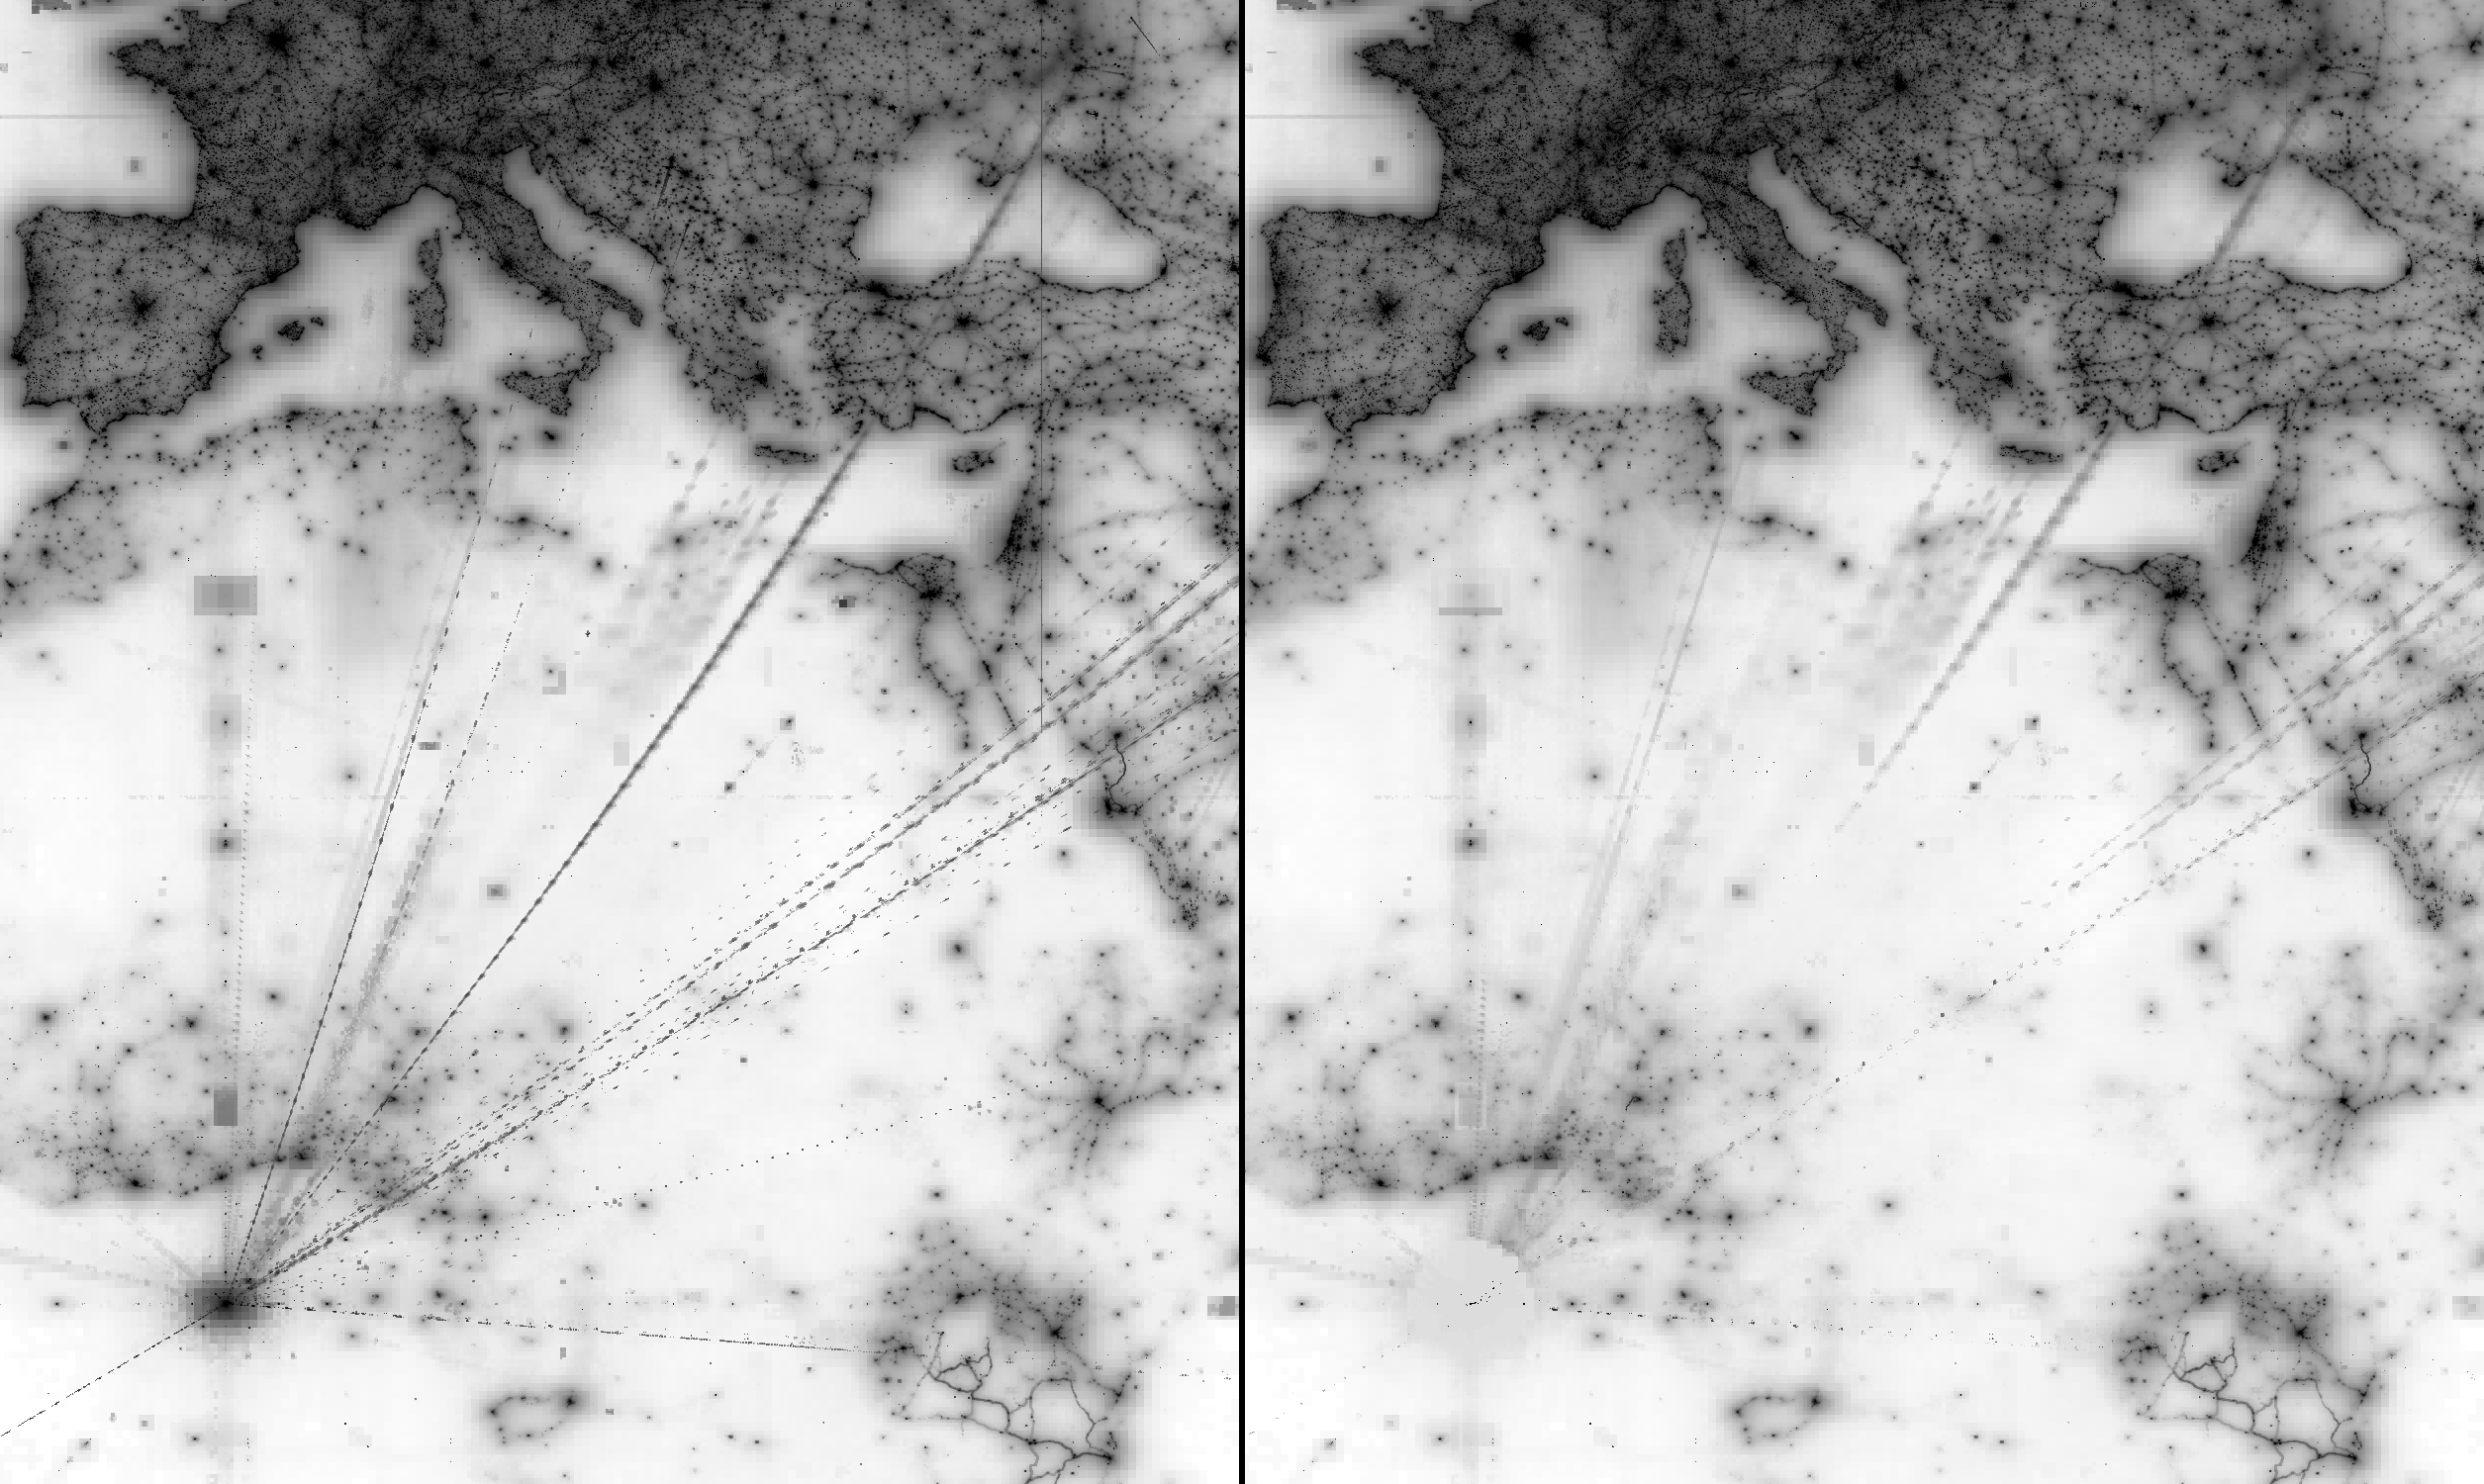
\includegraphics[width=\textwidth,alt={Two maps of Africa and Europe side
    by side. Left, the regular raster, with straight lines of dots fanning
    out from the Gulf of Guinea. Right, the filtered raster, where the lines
    are much fainter.}]{generated/fan.png}
  \caption{Lanes fanning out from Null Island over Africa and Europe, in the
    regular (left) and the filtered raster (right).
    \todo{Say which weeks once the release is pinned.}}
  \label{fig:fan}
\end{figure*}

\begin{figure}[t]
  \centering
  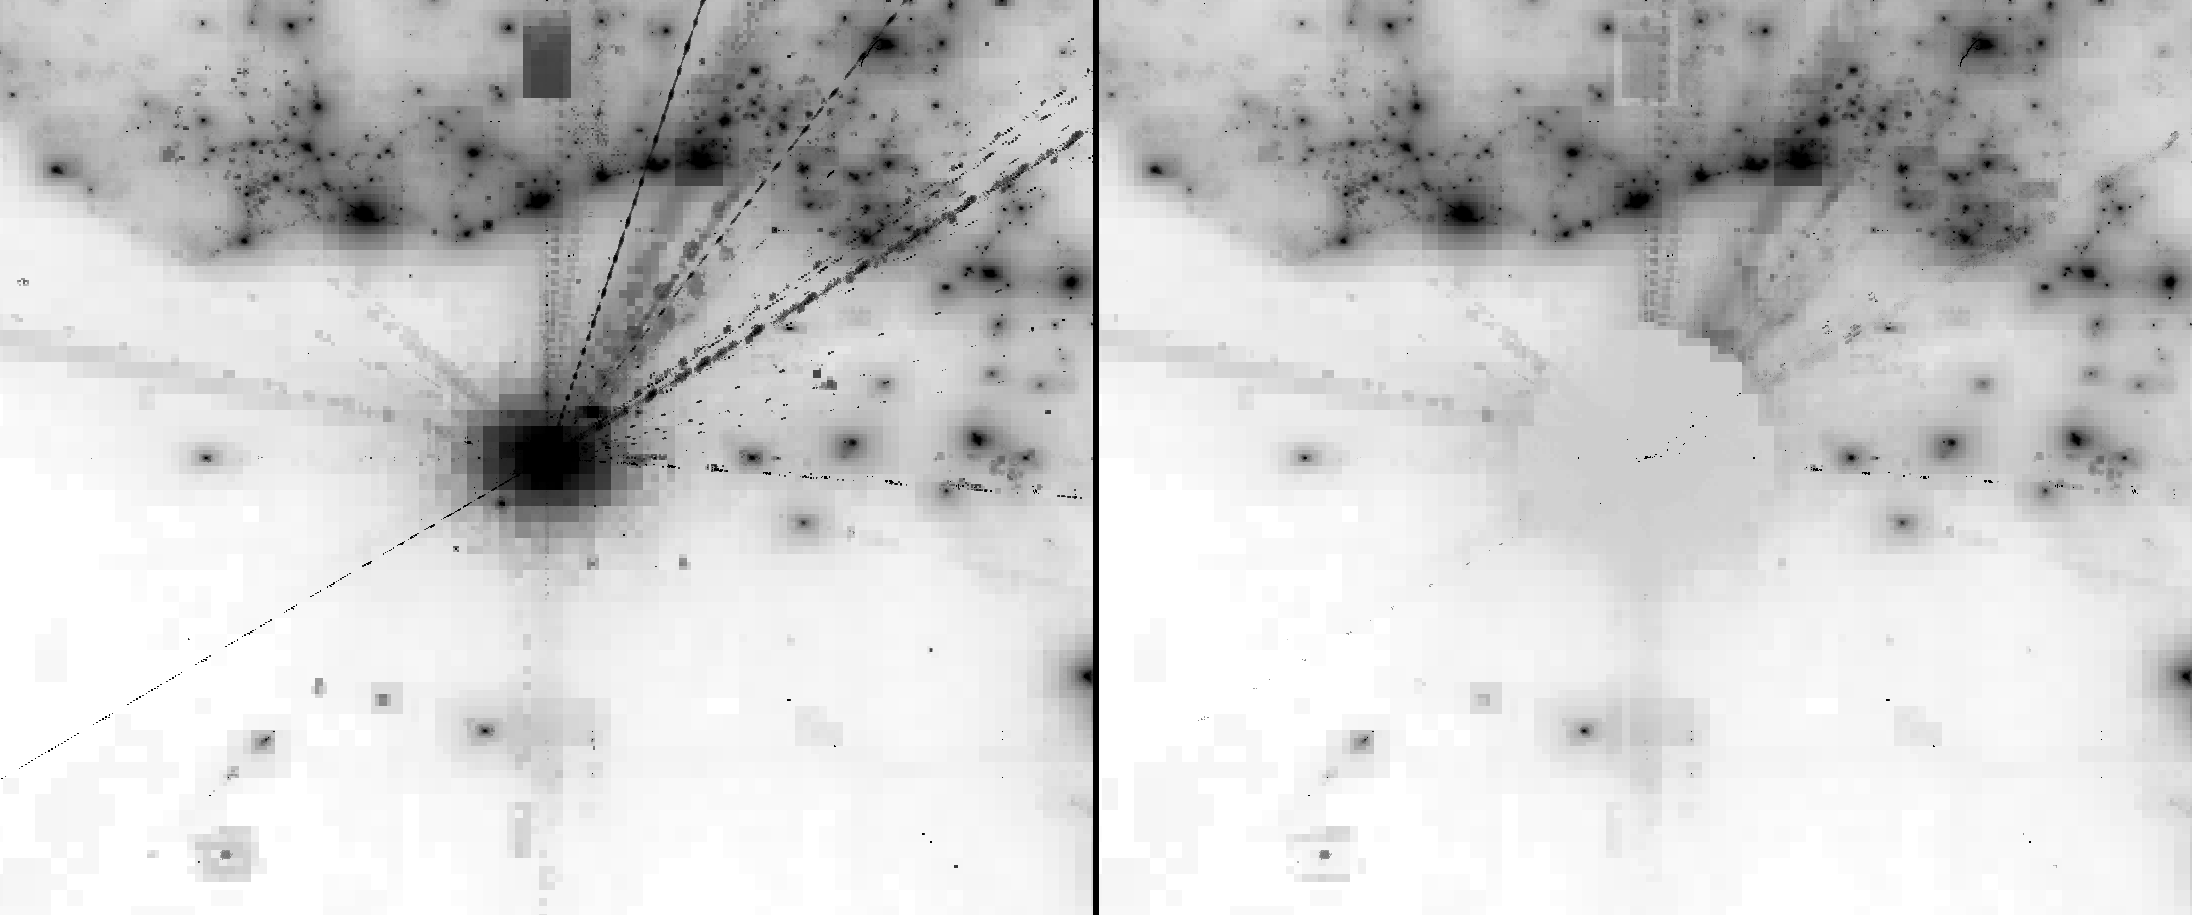
\includegraphics[width=\columnwidth,alt={Two maps of the sea around Null
    Island. Left, the regular raster with a bright spot of requests. Right,
    the filtered raster, where the spot is replaced by a uniform background
    matching the surrounding sea.}]{generated/null-island.png}
  \caption{Null Island, regular (left) and filtered (right). Tiles within
    3\textdegree{} are lowered to the background of the surrounding ring.}
  \label{fig:null-island}
\end{figure}

%========================================================================
\section{Data records}\label{sec:records}
\todo{Files and where to get them: the weekly GeoTIFF, the CycloneDX bill of
materials, datapackage.json, the experimental filtered GeoTIFF. Format
details: Cloud-Optimized GeoTIFF, Web Mercator, 256-pixel tiles, float32,
embedded histogram. Licence (CC0). Update cadence and retention.}

%========================================================================
\section{Technical validation}\label{sec:validation}

\subsection{Effect of the filter}
At the overview level of \resAgreementLevel{} pixels across the world,
the filter changes \resAgreementChanged{} of the \resAgreementPixels{} pixels
with views outside Null Island (\resAgreementChangedPct\,\%). The rank
correlation between the regular and the filtered raster over those pixels is
\resAgreementSpearman{} (Spearman).
\todo{Interpret: which pixels change (lanes, low-density sea and desert),
and why the correlation is lower than one might expect.}

\subsection{Injection test}
\todo{A known lane from one week injected into another; share of the lane
that survives, and real traffic removed elsewhere.}

\subsection{Agreement with other data}
\todo{Rank correlation at matched resolution with GHSL population, VIIRS
night lights, OpenStreetMap node density, and Wikimedia Commons photo
locations; regular vs.\ filtered.}

\subsection{Downstream use}
\todo{QRank: rank correlation for items with coordinates, lane items vs.\ a
matched control set. OSMDiffs: whether OSMViews helps rank edit proposals.}

\subsection{Stability and coverage}
\todo{Week-to-week stability; coverage compared with internet use by
country; effect of partial weeks.}

%========================================================================
\section{Usage notes and limitations}\label{sec:usage}
\todo{What the values mean and do not mean; bias toward users of the
standard tile servers; no individual data; overview levels are maxima, so
sums over them are not view counts.}

%========================================================================
\section{Code availability}\label{sec:code}
The builder, the artifact filter and this paper's evaluation are in
\url{https://github.com/brawer/osmviews}, under \code{cmd/osmviews-builder}
and \code{eval}. \code{make -C eval} downloads the pinned inputs listed in
\code{eval/inputs.toml} and regenerates every number and data figure in this
paper. \todo{Archive inputs and outputs on Zenodo and cite the DOI.}

\begin{thebibliography}{9}\small
\bibitem{defpub} S.~Brawer, \enquote{Method for memory-bounded construction
  of a globally complete, high-zoom-level Cloud-Optimized GeoTIFF from
  tile-access logs,} Technical Disclosure Commons, 2026.
  \url{https://www.tdcommons.org/dpubs_series/11589}
\bibitem{tilelogs} OpenStreetMap Foundation, tile-access logs.
  \url{https://planet.openstreetmap.org/tile_logs/}
\bibitem{density} M.~Ruthe (tyr\_asd), \enquote{OpenStreetMap node density
  map,} 2026. \url{https://www.openstreetmap.org/user/tyr_asd/diary/19549}
  \todo{Check author name and year.}
\end{thebibliography}

\end{document}
